\section{Optimal Green's function}
As it is apparent from \autoref{eq:p3m}, the method's validity depends on how well the mesh force approximates the reference force.
The average deviation between the two forces can be minimized by a suitable choice of Green's function given (in $k$ space) by
\begin{equation}\label{eq:optimal-greens-func}
    \hat{\mathcal{G}}(\mathbf{k}) = \frac{\mathbf{\hat{D}}(\mathbf{k}) \cdot \sum_{\mathbf{n}}\hat{U}^2(\mathbf{k_\mathbf{n}}) \mathbf{\hat{R}}(\mathbf{k}_\mathbf{n})}{|\mathbf{\hat{D}}(\mathbf{k})|^2 \left[ \sum_{\mathbf{n}}\hat{U}^2(\mathbf{k}_\mathbf{n}) \right]^2}.
\end{equation}
The derivation is mathematically involved and is detailed in \cite{Hockney1988}.
We now proceed to examine the terms appearing in \autoref{eq:optimal-greens-func}.

\subsection{Finite difference operator}
The Fourier transform $\mathbf{\hat{D}}$ of the two-point finite difference operator defined in \autoref{eq:two-point-central-diff} has the components
\begin{align*}
    \hat{D}_j(\mathbf{k})
     & = \int D_j(\mathbf{x}) e^{-i\mathbf{k}\cdot \mathbf{x}} d\mathbf{x}                                                                                                                                      \\
     & = \frac{1}{2H}\left( \int \delta(\mathbf{x} + H\mathbf{e}_j)e^{-i \mathbf{k}\cdot \mathbf{x}} d\mathbf{x} - \int \delta(\mathbf{x} - H\mathbf{e}_j)e^{-i \mathbf{k}\cdot \mathbf{x}} d\mathbf{x} \right) \\
     & = \frac{1}{2H} (e^{ik_j H} - e^{-ik_j H})
    = \frac{i \sin(k_j H)}{H}.
\end{align*}
Similarly, for the four-point finite difference (\autoref{eq:four-point-central-diff}) we have
\begin{equation*}
    \hat{D}_j = \alpha\frac{i\sin k_j H}{H} + (1- \alpha)\frac{i\sin 2k_j H}{2H},
\end{equation*}
where $j=1,2,3$.

\subsection{Assignment function}
The quantity $\hat{U}$ is defined as $\hat{W}/V$.
For the mass assignment scheme hierarchy described in \autoref{sec:mass-assignment} we have
\begin{equation*}
    \hat{U}(\mathbf{k}) = \left(\prod_{i=1}^{3}\frac{\sin(k_i H / 2)}{k_i H / 2}\right)^{p},
\end{equation*}
where $p=1,2,3,\dots$ with $p=1$ corresponding to NGP assignment, etc.
In particular, for the TSC assignment scheme, the \textit{alias sum}\footnote{
    To get the alias sums compatible with the DFT definition given in \autoref{eq:standard-dft}, one has to compute
    \begin{equation*}
        \sum_{\mathbf{n}} \tilde{U}^2(\mathbf{k}_\mathbf{n})
        \equiv \sum_\mathbf{n}\tilde{U}^2(\mathbf{k}+\mathbf{n}N)
        = \frac{1}{H}\sum_\mathbf{n}\hat{U}^2\left(\mathbf{k}\frac{2\pi}{NH}+\mathbf{n}\frac{2\pi}{H}\right)
    \end{equation*}
    instead.
}
\begin{equation*}
    \sum_{\mathbf{n}}\hat{U}^2(\mathbf{k}_\mathbf{n})
    \equiv \sum_{\mathbf{n}}\hat{U}^2\left(\mathbf{k} + \mathbf{n}\frac{2\pi}{H}\right)
\end{equation*}
can be rewritten as
\begin{align*}
    \sum_{\mathbf{n}} \hat{U}^2\left(\mathbf{k}+\mathbf{n}\frac{2\pi}{H}\right)
     & = \sum_{\mathbf{n}} \prod_{i=1}^{3} \left[ \frac{\sin(k_i H/2 + n_i\pi)}{k_i H/2 + n_i\pi} \right]^6 \\
     & = \prod_{i=1}^{3} \sum_{n_i} \left[ \frac{\sin(k_i H/2 + n_i \pi)}{k_i H/2 + n_i \pi} \right]^6      \\
     & = \prod_{i=1}^{3} \left[ \sin^6\left(\frac{k_i H}{2}\right)
        \sum_{n_i} \frac{1}{(k_i H/2 + n_i \pi)^6} \right]
\end{align*}
Using the partial fractions expansion of the cotangent function \cite{aigner2018proofs},
\begin{equation*}
    \frac{(-1)^s}{s!}\frac{d^s}{dx^s}\cot x = \sum_{n=-\infty}^{\infty} \frac{1}{(x-n\pi)^{s+1}},
\end{equation*}
we can simplify the sum over $n_i$ to
\begin{equation*}
    \frac{-1}{5!} \frac{d^5}{dx^5}\cot\left( \frac{k_i H}{2} \right)
    = 1 - \sin^2\frac{k_i H}{2} + \frac{2}{15}\sin^4\frac{k_i H}{2}.
\end{equation*}
Hence,
\begin{equation*}
    \sum_{\mathbf{n}}\hat{U}_\text{TSC}^2(\mathbf{k}_\mathbf{n})
    = \prod_{i=1}^{3} \left(1 - \sin^2\frac{k_i H}{2} + \frac{2}{15}\sin^4\frac{k_i H}{2}\right).
\end{equation*}
Using the same approach, we can obtain similar results for the CIC and NGP schemes, namely
\begin{equation*}
    \sum_{\mathbf{n}}\hat{U}_\text{CIC}^2 = \frac{1}{27} \prod_{i=1}^{3} \left(1 + 2\cos^2\frac{k_i H}{2}\right)
    \quad \text{and} \quad
    \sum_{\mathbf{n}}\hat{U}_\text{NGP}^2 = 1.
\end{equation*}

\subsection{Reference force}
The quantity $\mathbf{\hat{R}}$, the transformed reference force, is related to the shape $S$ of the particle-cloud by
\begin{equation}\label{eq:reference-force-transform}
    \mathbf{\hat{R}}(\mathbf{k}) = \frac{i\mathbf{k}\hat{S}^2(k)}{k^2},
\end{equation}
where $k = |\mathbf{k}|$.
This can be shown by recalling that $\mathbf{R}(\mathbf{x}_i - \mathbf{x}_j)$ is the force applied to cloud $i$ due to cloud $j$.
Hence, $\mathbf{R}(\mathbf{x})$ is the force on the cloud centered at $\mathbf{x}$ due to a cloud at the origin.
The force acting on mass element $d\mathbf{x}' S(\mathbf{x}' - \mathbf{x})$ of the cloud centered at $\mathbf{x}$ is therefore
\begin{equation*}
    -G d\mathbf{x}'S(\mathbf{x}' - \mathbf{x}) \int d\mathbf{x}'' S(\mathbf{x}'')\frac{\mathbf{x}' - \mathbf{x}''}{|\mathbf{x}' - \mathbf{x}''|^3}
\end{equation*}
and the total force is
\begin{equation}\label{eq:reference-force-clouds}
    \mathbf{R}(\mathbf{x}) = -G \int d\mathbf{x}'S(\mathbf{x}' - \mathbf{x}) \int d\mathbf{x}'' S(\mathbf{x}'')\frac{\mathbf{x}' - \mathbf{x}''}{|\mathbf{x}' - \mathbf{x}''|^3}.
\end{equation}
The expression on the right-hand side of \autoref{eq:reference-force-clouds} is a double convolution, $\mathbf{R} = -S * (S * \mathbf{g})$, where $\mathbf{g}(\mathbf{x}) = \mathbf{x}/|\mathbf{x}|^3.$
The $x$-coordinate of $\mathbf{g}$ is $x/|\mathbf{x}|^3$ which coincides with $\partial h / \partial x$ for $h(\mathbf{x}) = -1/|\mathbf{x}|.$
The Fourier transform of $h$ is given in \cite{gelfand1964generalized} (p. 363):
\begin{equation*}
    \hat{h}(\mathbf{k}) = \frac{4\pi}{|\mathbf{k}|^2}.
\end{equation*}
The formula for the transform of a derivative yields
\begin{equation*}
    \hat{g}_x(\mathbf{k}) = \frac{4\pi i k_x}{|\mathbf{k}|^2}.
\end{equation*}
Applying the convolution theorem twice and factoring the constant $(-4\pi G)$ out of the Green's function in \autoref{eq:optimal-greens-func} leaves us with the desired \autoref{eq:reference-force-transform}.

Since the shapes $S$ are spherically symmetric, the calculation of $\hat{S}$ (appearing in \autoref{eq:reference-force-transform}) can be simplified.
The Fourier transform of $S$ is
\begin{equation*}
    \hat{S}(\mathbf{k}) = \int S(\mathbf{x}) e^{-i\mathbf{k} \cdot \mathbf{x}} d\mathbf{x}.
\end{equation*}
Observe that $\mathbf{k} \cdot \mathbf{x} = kr\cos\theta$, where $\theta$ is the angle between $\mathbf{k}$ and $\mathbf{x}$, and $r = |\mathbf{x}|$.
Since $S$ is invariant under rotations, $\theta$ can be chosen to be the angle between $\mathbf{x}$ and the $z$-axis.
Thus, the integral, rewritten in spherical coordinates, becomes
\begin{equation*}
    \hat{S}(k) = \int_{0}^{2\pi}d\phi \int_{0}^{\pi} d\theta \int_{0}^{\infty}dr S(r)e^{-ikr\cos\theta}r^2\sin\theta
    = 2\pi \int_{0}^{\infty} r^2 dr \int_{0}^{\pi} d\theta e^{-ikr\cos\theta} \sin\theta.
\end{equation*}
The $\theta$-integral upon the substitution $-kr\cos\theta \to u$ becomes
\begin{equation*}
    \frac{1}{kr}\int_{-kr}^{kr} e^{iu} du
    = \frac{1}{kr} \int_{-kr}^{kr} (\cos u + i \sin u) du
    = \frac{2\sin kr}{kr}
\end{equation*}
and hence
\begin{equation*}
    \hat{S}(k) = 4\pi \int_{0}^{\infty} r^2 S(r)\frac{\sin kr}{kr}dr.
\end{equation*}

This integral, evaluated for the $S_1$ and $S_2$ shapes respectively, gives
\begin{equation*}
    \hat{S_1}(k) = \frac{3}{(ka/2)^3} \left(\sin\frac{ka}{2} - \frac{ka}{2} \cos\frac{ka}{2}\right)
\end{equation*}
and
\begin{equation*}
    \hat{S_2}(k) = \frac{12}{(ka/2)^4}\left(2 - 2\cos\frac{ka}{2}-\frac{ka}{2}\sin\frac{ka}{2}\right).
\end{equation*}

Finally, we note that the infinite sum in the numerator of \autoref{eq:optimal-greens-func} does not have a closed form, but this does not pose a problem since the summand decays rapidly with $\mathbf{n}$ moving further away from zero.

The result of applying the optimal Green's function in \autoref{eq:poisson-fourier-product} is illustrated in \autoref{fig:reference-force-combined}\subref{fig:reference-force-approx-sub}.
As can be seen, the PM force closely follows the reference force, especially for distances \( r > a \), where the reference force nearly matches the inverse-square law.
It is worth noting that for \( r \) slightly smaller than \( a \), the reference force and its mesh-based PM approximation still provide a good fit to the inverse-square behavior.
This observation allows the cutoff radius \( r_e \), which defines the boundary for direct summation, to be chosen smaller than \( a \) (e.g., \( r_e = 0.7a \)), improving performance without sacrificing accuracy.
\begin{figure}[htp]
    \centering
    \begin{subfigure}[b]{0.48\textwidth}
        \centering
        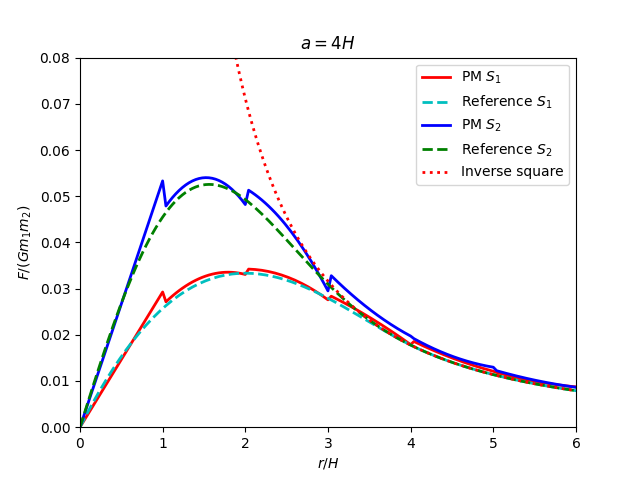
\includegraphics[width=\textwidth]{chapters/p3m-method/img/s1-vs-s2.png}
        \caption{Approximate vs. reference force.}
        \label{fig:reference-force-approx-sub}
    \end{subfigure}
    \hfill
    \begin{subfigure}[b]{0.48\textwidth}
        \centering
        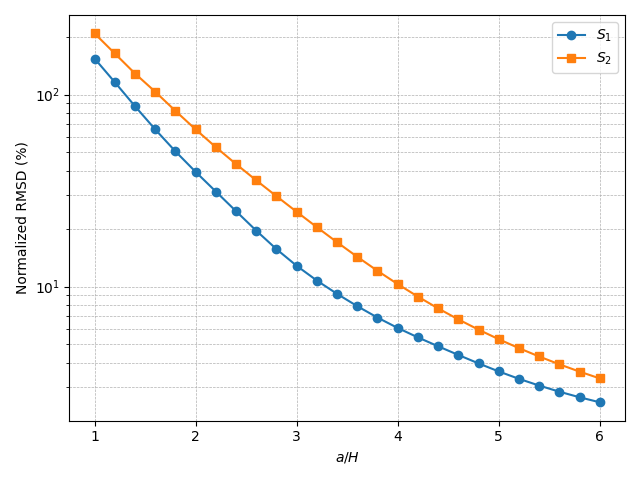
\includegraphics[width=\textwidth]{chapters/p3m-method/img/s1-vs-s2-nrmsd.png}
        \caption{Mean-normalized RMSD error}
        \label{fig:reference-force-error-sub}
    \end{subfigure}
    \caption{Comparison of PM approximation using $S_1$ and $S_2$ shape functions.
        The mesh approximation to the reference force was computed using the PM method with a TSC assignment scheme, two-point finite difference, and Green's function optimal for each shape.
    }
    \label{fig:reference-force-combined}
\end{figure}

\subsection{Error analysis}\label{subsec:p3m-error-analysis}
The \PThreeM{} method offers a high degree of flexibility in terms of specifying the ``building blocks'' of the Green's function in \autoref{eq:optimal-greens-func}.
For example, we can be interested in learning how the choice of the assignment scheme influences the shape of the PM-approximated reference force.
The result of a test that addresses this issue is shown in \autoref{fig:reference-force-approx-different-schemes}.
\begin{figure}[htp]
    \centering
    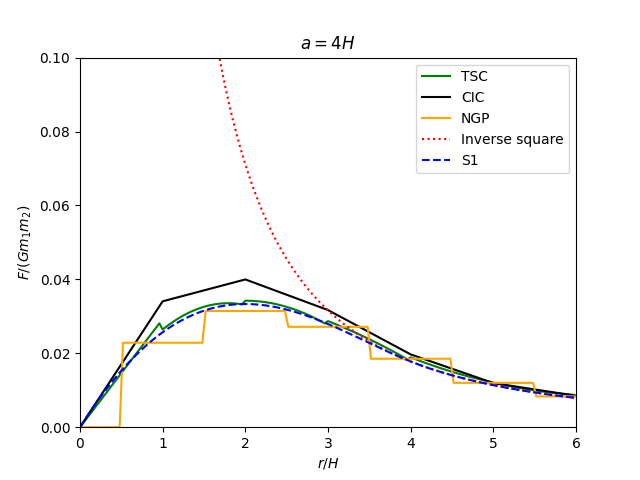
\includegraphics[scale=0.5]{chapters/p3m-method/img/field_different_ass.png}
    \caption{Approximate vs. reference force.}
    \label{fig:reference-force-approx-different-schemes}
\end{figure}
The figure shows that the general characteristic of the field strength approximated by the PM method is similar to what we have already seen in \autoref{fig:pm-mass-assignment-field-strength}.
Namely, the NGP scheme yields an unnatural, jagged shape.
The shape produced using the CIC shape matches the $S_1$ reference force more closely, although it overestimates the field strength values close to the source.
The most accurate approximation is obtained using the TSC scheme (this is the same shape we have already seen in \autoref{fig:reference-force-approx-sub}).


To measure the quality of PM-approximation of a given reference force, we used mean-normalized RMSD error, i.e., we calculated
\begin{equation*}
    \frac{\sqrt{\frac{1}{n} \sum_{i=1}^{n} (F^\text{PM}(r_i) - R(r_i))^2}}{\frac{1}{n} \sum_{i=1}^{n} R(r_i)}
\end{equation*}
in a system with a single unit mass located on the $x$-axis.
The forces $F^\text{PM}(r_i)$ were measured along the $x$-axis in equal-length intervals, and the test was run for increasing values of particle diameter $a$.
The result of the test is shown in \autoref{fig:reference-force-combined}\subref{fig:reference-force-error-sub}.
Clearly, the approximation error becomes smaller for increasing values of $a$.
Since $r_e$ is proportional to $a$, this implies that there is a trade-off between accuracy and the execution time.
Increasing $a$ means that $r_e$ should increase as well, which forces more particles into short-range correction regions.
If the system under consideration has uniform density, we note that for any given particle, the short-range correction is concerned with $\sim r_e^3$ particles in its vicinity, which translates into $\sim r_e^3$ operations.
The relation between cutoff radius size $r_e$ and execution time is shown in \autoref{fig:p3m-time-vs-radius}.
\begin{figure}[htp]
    \centering
    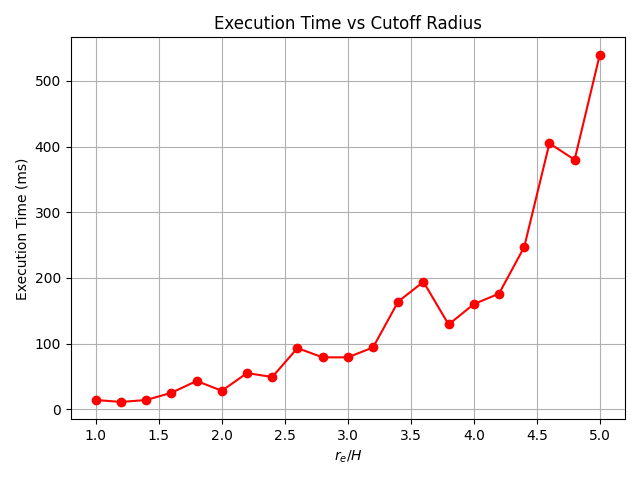
\includegraphics[scale=0.5]{chapters/p3m-method/img/time-vs-radius.png}
    \caption{Execution time for different setting of cutoff radius $r_e$ in the \PThreeM{} method (single step, $N=10{,}000$).
    The times shown in the graph do not include tabulating the Green's function and the PM step.}
    \label{fig:p3m-time-vs-radius}
\end{figure}
As we can see, the execution time very strongly depends on $r_e$, and this explains why choosing $r_e$ slightly, even slightly less than $a$, can lead to significant improvements in performance.
Another conclusion that can be drawn from \autoref{fig:reference-force-error-sub} is that the \( S_2 \)-based approximation exhibits higher mean-normalized RMSD error compared to \( S_1 \).
However, as we remarked previously, it allows for choosing $r_e \lesssim a$ without significant loss of accuracy.
Therefore, the choice between \( S_1 \) and \( S_2 \) shapes involves a trade-off between accuracy near the source and overall error, making the optimal choice context-dependent.

